\documentclass[12pt,a4paper]{article} %,fleqn
\usepackage{Diplo}
\usepackage[utf8]{inputenc} 
\usepackage[russian]{babel}

\usepackage[left=3cm,right=1.5cm,
top=2cm,bottom=2cm]{geometry}
\usepackage{longtable}
\usepackage{comment}
\usepackage{amsfonts}
\usepackage{hyperref}
\usepackage[square, comma, sort&compress, numbers]{natbib}
\newtheorem{definition}{Определение}
\newtheorem{theorem}{Теорема}
\newtheorem{utv}{Утверждение}

\graphicspath{{../pics/}}

\newcommand{\specialcell}[2][c]{%
	\begin{tabular}[#1]{@{}c@{}}#2\end{tabular}}

\begin{document}
	
\vskip 3mm

\setcounter{page}{1}
%%%%%%%% Титульный лист %%%%%%%%%%%%%%%%%%%%%%%%%%%%%%%%%
\begin{center}
	\thispagestyle{empty}
	
	{ Министерство науки и высшего образования Российской Федерации\\}

	
	
	{ Московский Физико-технический институт \\}
	
	{ (Государственный Университет) \\}
	
	{ Физтех-школа прикладной математики и информатики  \\}
	
	{ Кафедра технологий цифровой трансформации\\[4cm]}
	
	
	{ \bf \Large Выпускная квалификационная работа\\}
	
	{ \bf \Large{"Развитие инструментов предиктивной аналитики в целях повышения эффективности мониторинга проектов в сфере жилищного строительства"\\[1cm]} }
	
	{\bf {Студента 2-го курса Ефремова Сергея Владимировича}\\[3cm]}
	
\end{center}

\begin{flushright}
	\bf{Научный руководитель}\\
	\bf{кандидат экономических наук, доцент Помулев А. А.}\\[4cm]
\end{flushright}


\begin{center}
	Москва, 2022
\end{center}
%%%%%%%%%%%%%%%%%%%%%%%%%%%%%%%%%%%%%%%%%%%%%%%%%%%%%%%%%%%%%%%%

\newpage
\begin{abstract}

Рассматривается задача улучшения инструментов предиктивной аналитики, использующихся при мониторинге проектов в сфере жилищного строительства. Исследованы предложенные ранее схемы решения этой проблемы, на основе изученных материалов разработан подход по улучшению оценки вероятности просрочки выплаты займа застройщиком на основании отчетности, публикуемой в открытом доступе и уровне зависимости от импортируемых комплектующих и материалов. Предложен, реализован и протестирован алгоритм, основанный на алгоритмах нейросетевого обучения с использованием чисел Шепли.	

\end{abstract}

\newpage
\tableofcontents
 


\newpage
\section{Введение}


 

\newpage
\subsection{Цели и задачи работы}

\textbf{Цель и задачи исследования.} Целью исследования является построение модели предиктивной аналитики, которая позволит повысить эффективность процесса мониторинга проектов коммерческим банком в сфере жилищного строительства и улучшить качество прогнозирования вероятности просрочки платежа по сравнению с существующими моделями. Для реализации этой цели были поставлены следующие задачи:
\begin{itemize}
	\item изучить определение понятий: «мониторинг», «эффективность мониторинга», «предиктивная аналитика» для использования в настоящем исследовании;
	\item провести анализ существующих проектов и динамики их развития в сфере жилищного строительства;
	\item ознакомиться с текущим состоянием финансирования проектов в сфере жилищного строительства и нормативно-правовой базой;
	\item изучить процесс мониторинга проектов и методы их оценки коммерческим банком;
	\item исследовать типы моделей предиктивной аналитики и их применение в кредитном процессе;
	\item выделить основные проблемы процесса мониторинга проектов и определить возможности их решения с использованием инструментария предиктивной модели 
	\item разработать алгоритм внедрения разработанного инструментария в бизнес-процесс мониторинга
	\item рассчитать экономический эффект от внедрения модели 
\end{itemize}

\bigskip

\textbf{Научная новизна.} Используется нейросетевой подход к определению вероятности банкротства заемщика с выделением признаков, вносящих максимальный вклад с помощью, чисел Шепли. В работе предлагается коэффициент, позволяющий оценить зависимость застройщика от импортных комплектующих и материалов, а также уровень потенциального риска, обусловленного политическими ограничениями.

\bigskip

\textbf{Методы исследования.} Алгоритмы реализованы на языке программирования Python с использованием библиотек |||.

\bigskip

\textbf{Практическая ценность.} Полученная модель может быть использована в качестве встраиваемого модуля. Например, с её помощью можно:
\begin{itemize}
	\item корректировать оценку вероятности просрочки платежа застройщиком, учитывая его зависимость от импортируемых компонентов;
	\item дополнять существующие системы мониторинга объектов строительства показателем уровня зависимости от импортных компонентов и моделью оценки наиболее важных показателей, влияющих на просрочку.
\end{itemize}
%%%%%%%%%%%%%%%%%%%%%%%%%%%%%%%%%%%%%%%%%%%%%%%%%%%%%


\newpage
\section{Постановка задачи}


\subsection{Мониторинг проектов}\label{task}

изучить определение понятий: «мониторинг», «эффективность мониторинга», «предиктивная аналитика» для использования в настоящем исследовании

Мониторинг проекта - процесс измерения показателей выполнения проекта, сбора данных об исполнении проекта, информационного обслуживания управления проектом с целью выявления его соответствия желаемому результату и плану, с последующим представлением и распространением полученных данных.

Под контролем проекта понимается процесс сравнения фактических значений контрольных показателей с запланированными, последующего анализа отклонений, оценки тенденций и прогнозирования возможных альтернатив, разработки корректировок хода реализации проекта для улучшения прогноза.

Основными целями контроля и мониторинга инвестиционных проектов можно считать обеспечение:
\begin{itemize}
	\item своевременного достижения целей проекта с учетом согласованной стоимости;
	\item срочности, возвратности, платности и целевого использования предоставляемых банком кредитных ресурсов для финансирования проекта;
	\item своевременного информирования руководства банка о выявленных проблемах, прогнозирования рисков реализации проекта и разработка мер по их снижению;
	\item достижения заложенных в проекте показателей социально-экономической эффективности.  
\end{itemize}

Чаще всего при реализации проектов в сфере жилищного строительства выделяют следующие виды мониторинга:
\begin{itemize}
	\item мониторинг хода реализации инвестиционного проекта (сроков выполнения работ, бюджета проекта, расчетного времени окончания работ и расчетной стоимости проекта, организация технадзора и контрольных проверок);
	\item финансовый мониторинг (финансово-экономического состояния заемщика, исполнителя проекта, поручителей, гарантов, обеспечения по кредиту/кредитной линии; денежного потока, коэффициентов покрытия, целевого использования средств, исполнения заемщиком обязательств перед банком);
	\item мониторинг эффективности инвестиционного проекта (показателей, которые предусмотрены положением об экспертизе проектов банка).
\end{itemize}

Такое разделение обуславливается необходимостью не только контролировать текущую операционную деятельность, ведущуюся по проекту, исполнение финансовых обязательств участниками проекта и целевое использование средств, но и конечные результаты этой деятельности, которые выражаются в достижении целей проекта и достигнутой социально-экономической значимости.

Основными элементами систем мониторинга инвестиционных проектов являются:
\begin{itemize}
	\item финансовая, техническая и иная отчетность заемщика;
	\item экспертные оценки банковских специалистов по направлениям реализации проекта, независимые эксперты (технический надзор, финансовый аудит);
	\item календарно-сетевые графики работ, расчеты сроков ввода объекта в эксплуатацию и суммарной стоимости работ;
	\item данные автоматизированных информационных систем мониторинга инвестиционных проектов.
\end{itemize}

Последние и будут рассмотрены в первую очередь в данной работе.

Ключевые этапы мониторинга проектов:
\begin{itemize}
	\item этап подготовки проекта (начинается с момента одобрения займа/кредитной линии и заканчивается выделением финансовых средств);
	\item инвестиционная стадия проекта (непосредственное финансирование проекта);
	\item этап эксплуатации (следует до полного исполнения заемщиком платежных обязательств перед банком).
\end{itemize}

\subsection{Эффективность мониторинга}

Построением эффективных систем мониторинга занимались многие исследователи Д. Боуэр, Дж.Филлипс, Р.Фартел, Х.Керцнер[здесь будут ссылки на литературу]. Мониторинг в современных реалиях представляет из себя комплексную функцию проектного управления, в которую входит процедуры сбора, анализа и передачи информации о ходе реализации проекта, которая позволяет решить проблему своевременного принятия решений по проекту.

Основные задачи, которые решают системы мониторинга:
\begin{itemize}
	\item определение совокупности отслеживаемых индикаторов;
	\item организация обработки и агрегирования полученной информации;
	\item генерация текущей отчетности по проекту;
	\item интеграция функции мониторинга в информационную архитектуру предприятия, реализующего проект.
\end{itemize}

Принятие управленческих решений о формировании и развитии системы мониторинга проектов,о требуемом кадровом, техническом и финансовом обеспечении неизбежно связано с дополнительными затратами. Однако, потенциальные угрозы от финансирования убыточных или высокорисковых проектов также способны привести к значительным издержкам. Все это остро ставит вопрос о необходимости эффективного мониторинга проектов.

Основными подходами к изучению эффективности проектов являются:
\begin{itemize}
	\item целевой (предполагает анализ степени достижения целевых значений показателей);
	\item динамический (учитывает скорость изменения исследуемых показателей во времени и относительно друг друга);
	\item затратный (основан на сопоставлении затрат и результатов);
	\item ресурсный (исследует степень рациональности расходования ресурсов).
\end{itemize}

\subsection{Предиктивная аналитика}

Предиктивной аналитикой или продвинутой аналитикой называют ряд аналитических и статистических методов прогнозирования действий и поведения в будущем. В основе лежат статистические модели, позволяющие находить закономерности в исторических и транзакционных данных, что позволяет выделять потенциальные риски и возможности. Ключевые этапы составляющие процесс предиктивного анализа: подключение к данным, анализ и визуализация результатов исследований, развитие предложений и моделей данных, применение предиктивных моделей, оценка и прогнозирование будущих результатов.

В основе предиктивной аналитики лежит выявление связей между данными историческими и прогнозными результатами на их основе. Верхнеуровнево алгоритмы предиктивного анализа можно разделить на контролируемое и неконтролируемое обучение.

Контролируемое обучение принято разделять на две ключевые категории: регрессию для количественных ответов и классификацию для определения фактической принадлежности ответа к той или иной группе. 
 
Неконтролируемое обучение применяется для получения выводов из входных данных без разметки. Наиболее распространенный вид такого анализа - кластеризация, которую используют для поиска скрытых закономерностей в данных.

%%%%%%%%%%%%%%%%%%%%%%%%%%%%%%%%%%%%%%%%%%%%%%%%%%%%%

\newpage
\section{Обзор действующей практики}
\subsection{Анализ текущего состояния рынка жилищного строительства и тенденции развития}

В "Стратегии строительной отрасли до 2030 года" особое внимание уделяется наращиванию жилищного строительства, а также повышению комфортности жилищных условий. Так, в разделе "Целевые показатели по ипотеке и жилищному строительству" документа сформулирована задача увеличить обеспеченность населения жильем к 2024г. до $28-30~\text{м}^2$ на человека в среднем, а к 2030 году превысить этот уровень. Также предполагается повысить долю городов с благоприятной городской средой до 70\% к 2030г. Для того, чтобы достичь поставленных целей, необходимо нарастить объем жилищного строительства до не менее чем 120 млн.$~\text{м}^2$ в год (рис.~\ref{fig:develop_dynam}).

\begin{figure}[h]
	
	\centering
	
	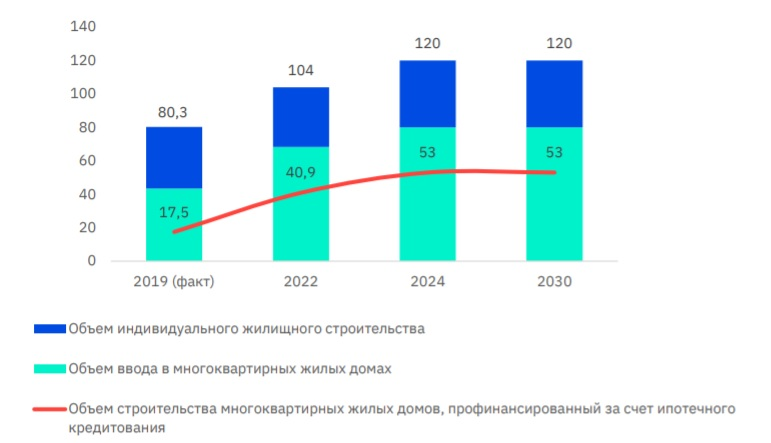
\includegraphics[width=0.7\linewidth]{develop_dynam.jpg}
	
	\caption{Классификация источников финансирования девелоперского проекта в зависимости от стадии его реализации.}
	
	\label{fig:develop_dynam}
	
\end{figure}

На 21 апреля 2022г. в процессе строительства находится около 95 млн.~$\text{м}^2$ и только строительство 3,5\% от суммарной площади финансируется без привлечения средств граждан.[дом.рф]
 
Количество действующих договоров проектного финансирования на 1 марта 2022 года - 5273 по всей России.[ЦБ] Общая сумма действующих кредитных договоров - 7 813 578,8 млн. рублей.
Рост за год по сравнению с данными на 1 марта 2021 года - на 96\% по количеству, и на 139\% по объему.
При этом на Москву и Московскую область приходится около 20\% заключенных договоров, сумма которых составляет 57\% от всех выданных займов. То есть можно говорить о существенном перевесе в пользу Московского региона, относительно всей России и высоких темпах роста рынка, и в Московском регионе в частности. Однако, к сожалению, не все объекты строительства одинаково успешны и есть тенденция роста проблемных проектов. Так в реестре проблемных застройщиков числятся – 650 организаций в 66 регионах РФ. И на фоне ограниченности ресурсов, сбоя налаженных логистических поставок и роста ставок по кредитам этот реестр будет только пополняться. В частности поэтому, сейчас, как никогда, банку важно вовремя выявить проблемного застройщика и успеть принять превентивные меры, до того как он перестанет платить по счетам или не сможет далее вести деятельность.  

\subsection{Текущее состояние финансирования в сфере жилищного строительства}

\subsubsection{Основные источники финансирования }

В общемировой практике недвижимость считается одним из наименее рисковых направлений долгосрочного инвестирования с достаточно высоким уровнем рентабельности. Однако условия доступа, задающиеся высоким уровнем капитальным затрат, ограничивают круг потенциальных инвесторов. Так как крупные девелоперские проекты нуждаются в крупных капиталовложениях, реализация их за счет исключительно собственных средств для большинства компаний оказывается невозможной. Однако учитывая текущую практику, именно внешнее финансирование как нельзя лучше отражает суть девелопмента.
В зависимости от стадии реализации девелоперского проекта основные источники финансирования могут быть классифицированы в соответствии со схемой (рис.~\ref{fig:fin_source_clas}). 

\begin{figure}[h]
	
	\centering
	
	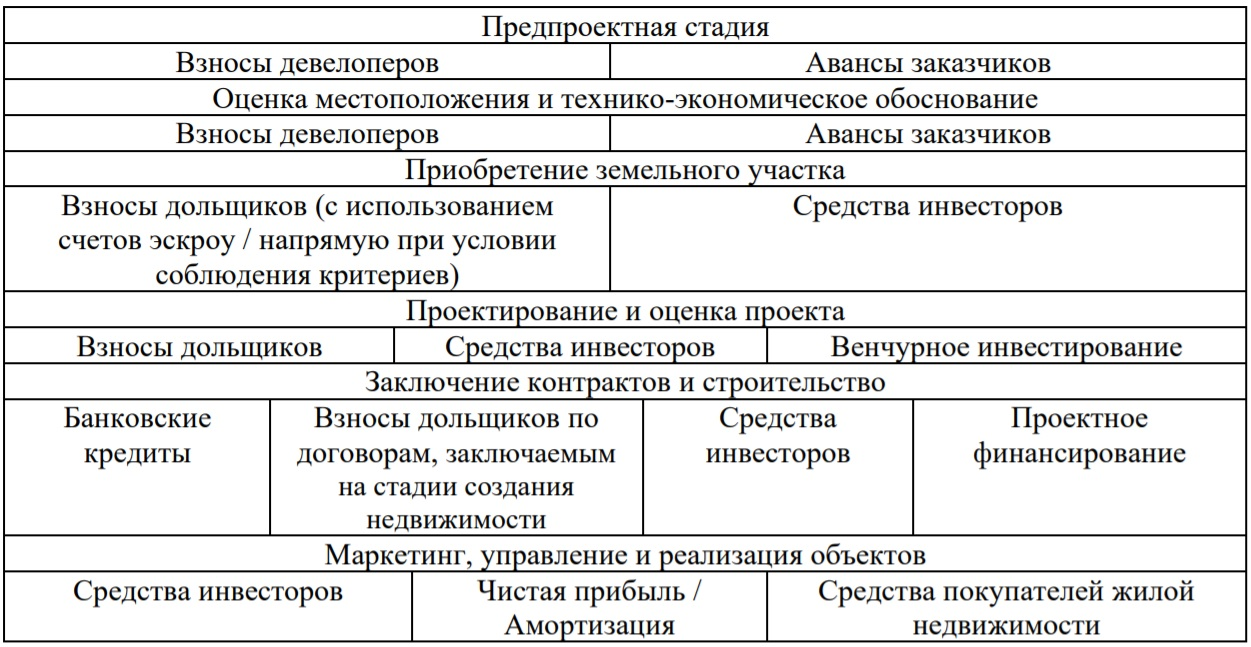
\includegraphics[width=0.7\linewidth]{fin_source_clas.jpg}
	
	\caption{Классификация источников финансирования девелоперского проекта в зависимости от стадии его реализации.}
	
	\label{fig:fin_source_clas}
	
\end{figure}

На первых этапах, как на самых рисковых, проект в основном финансируется за счет собственных средств. Далее, когда конфепция будущего объекта строительства уже разработана, привлекаются средства дольщиков. Финансирование проекта на стадии приобретения земельного участка носит рисковый характер, поэтому инвестиционные ресурсы оказываются самыми дорогими.

На этапе строительства используются банковские, облигационные займы и эскроу-счета. Этот этап проекта наиболее капиталоемкий  и требует значительных объемов инвестиционных ресурсов. На стадии продвижения привлечение заемных средств оказывается невозможным, так как займы выдаются под строительство.
В условиях Российского рынка задача усложняется высокими ценами на земельные участки, строительные материалы, значительными транспортными расходами и прочими издержками.

Наиболее распространенные механизмы рыночного финансирования девелоперских проектов в России:
\begin{itemize}
	\item договоры купли-продажи объектов жилой недвижимости;
	\item договоры участия в долевом строительстве;
	\item эскроу-счета.
\end{itemize}

До 2019 года наиболее распространенным механизмом финансирования было заключение договора участия в долевом строительстве (ДДС). Так на конец 2019 года в России было зарегистрировано 783 тысячи договоров ДДС. Такая популярность обусловлена рядом факторов[]: для покупателя - покупка на начальных этапах строительства позволяла сэкономить 25-35\% от стоимости готового объекта; использование инструментов снижения рисков, в частности государственная регистрация ДДС, страхование; в ряде случаев договоры предусматривали рассрочку платежей. Однако данный механизм имел ряд недостатков, в частности порожденная им проблема обманутых дольщиков. 
Для решения проблемы был разработан комплексный ряд мер, а именно были внесены правки в Федеральный закон от 30.12.2004г. №214-ФЗ "Об участии в долевом строительстве многоквартирных домов и иных объектов недвижимости и о
внесении изменений в некоторые законодательные акты Российской
Федерации". Как результат - с 1 июля 2019 года в России осуществляется переход на новую схему финансирования строительства многоквартирных домов через эскроу-счета.

\subsubsection{Эскроу-счета}

При применении данного подхода застройщик финансирует проект за счет собственных средств и банковских кредитов, а деньги дольщиков за проданные квартиры, хранящиеся на эскроу-счетах,  получает после сдачи проекта в эксплуатацию. 

По данным Банка России, уже на начало сентября 2020г. в банках было открыто почти 180 тыс счетов эскроу, на которых аккумулированно более 600 млрд. руб. При этом банки одобрили финансирование на 1,8 трлн руб., при общем объеме ссудной задолжности 667 млрд руб. А по состоянию на 1 марта 2022 года количество эскроу-счетов составило более 681 тыс, при объеме аккумулированных на этих счетах средств более 3,39 трлн. рублей. 
По данным Банка России, средняя процентная ставка кредитной линии проектного финансирования составляла 4-6\% для договоров, заключенных до марта 2022 года. Средний срок рассмотрения заявки 30-45 дней. Особенность кредитования с применением счетов-эскроу заключается в том, что при значительном размере поступлений денежных средств участников долевого строительства на счета эскроу - ставка по кредиту снижается, в пределе она может быть снижена до 0.01\%.

\begin{figure}[h]
	
	\centering
	
	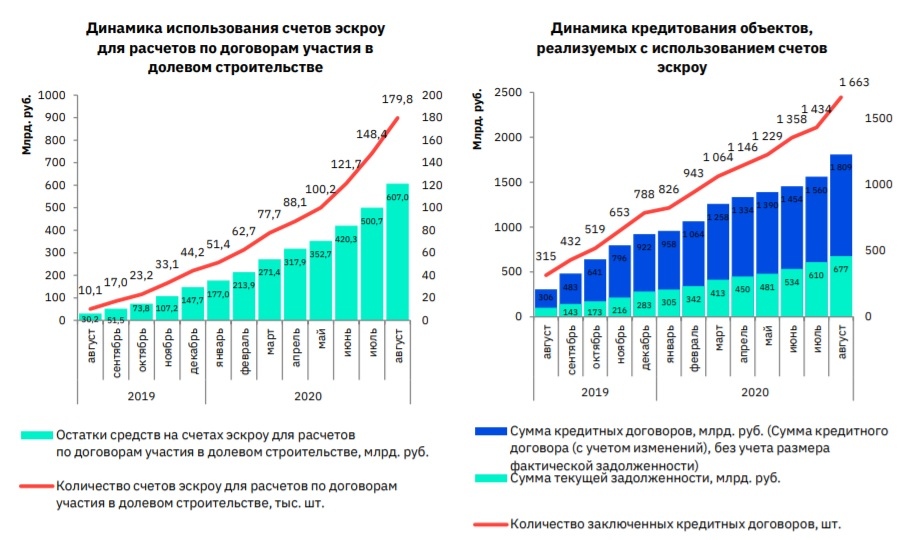
\includegraphics[width=0.7\linewidth]{eskrou_dynam.jpg}
	
	\caption{Динамика использования экроу счетов.}
	
	\label{fig:eskrou_dynam}
	
\end{figure}

Переход на новую модель финансирования жилищного строительства сопряжен с решением ряда систематических проблем. В первую очередь, данная модель предполагает замену средств дольщиков банковским кредитованием. Согласно расчетам ДОМ.РФ, для этого потребуется увеличение объемов кредитования застройщиков с 0,6 трлн руб. в 2018 г. до 6,4 трлн руб. в 2024 г. То есть на горизонте 4-5 лет, кредитный портфель застройщиков жилой недвижимости должен возрасти примерно в 10 раз(рис.~\ref{fig:eskrou_dynam}).

Обслуживание ссудной задолженности в рамках новой модели финансирования строительства жилой недвижимости возможно только при условии растущих объемов продаж квартир на первичном рынке. Основным драйвером спроса при этом считается развитие ИЖК и его льготных программ, субсидируемых государством. По итогам 2019 г. примерно 60\% квартир в новостройках и 50\% на вторичном рынке приобретены с помощью ИЖК.
Основными ограничителями спроса выступают повышение долговой нагрузки вследствие отставания динамики денежных доходов от платежей по кредиту и рост цен жилой недвижимости. Особенно остро обе эти проблемы ощутились на фоне повышения ключевой ставки ЦБ до 20\% в марте, ставки по ИЖК стали неподъемными даже по льготным программам ипотечного кредитования, а цены на недвижимость продолжили рост на фоне повысившихся инфляционных ожиданий национальной валюты.

Реформа отрасли строительства жилой недвижимости оставила девелоперов без возможности использовать бесплатные средства дольщиков. На начальных этапах перехода на проектное финансирование объем жилищного строительства в РФ снизился на 20 млн кв.м. Половина регионов Российской Федерации характеризуется нулевой или отрицательной маржинальностью жилищного строительства, обусловленной низкой платежеспособностью населения. Все это ограничивает застройщика при выборе источников финансирования. Также важен и тот факт, что кредит не покрывает все затраты проекта, а собственных средств застройщика может быть недостаточно для увеличения объема строительства. 

Для поддержания темпов роста, застройщики выходят на фондовый рынок. Доверие потенциальных инвесторов к ценным бумагам строительных компаний потенциально могут повысить структурирование девелоперских групп,  цифровизация компаний, повышение прозрачности их отчетности и формирование рейтинговой истории. Однако в связи со сложной политической обстановкой, правильно будет ориентироваться на привлечение  инвесторов внутри страны, так как доступ внешнего капитала весьма ограничен. Также исключительно важной становится и степень зависимости застройщика от внешнего капитала и импортных комплектующих, материалов и инструментов при строительстве. Чем выше степень зависимости, тем менее устойчивой становится девелопер и конкретные, финансируемые банком проекты, при оказании на них даже косвенного политико-экономического давления.

Все это приводит к необходимости постоянного проектного мониторинга и контроля потенциальных рисков со стороны банка, как у регулятора на новом сложившемся рынке жилищного строительства после введения счетов-эскроу.
  

\subsection{Процесс мониторинга проектов и методы оценки коммерческим банком}

Мониторинг коммерческим банком хода реализации проекта состоит из:
\begin{itemize}
	\item разработки календарно-сетевого графика создания объектов инвестиционного проекта и пояснения к нему;
	\item организации контроля за соблюдением плановых сроков, этапов, стоимостных параметров; назначением платежей; а также фактически выполненного объема работ и освоенных затрат на всех стадиях реализации проекта;
	\item выявления отклонений от плана реализации проекта и их последующего анализа, в том числе оценку влияния на сроки и бюджет проекта;
	\item разработки мер, направленных на снижение влияния отклонений, для выполнения проекта в запланированные сроки с установленным бюджетом;
	\item прогнозирования сроков окончания реализации проекта и суммарных затрат
	\item мониторинга исполнения дополнительных обязательств, в том числе организации и осуществления контроля над выполнением заемщиком, залогодателем и поручителями дополнительных условий и обязательств, установленных договором;
	\item организации экспертизы бюджетного проекта и проверки соответствия стоимостных параметров проекта текущему состоянию рынка строительных материалов, работ и оборудования;
	\item организации оперативного надзора за техническими и объемно стоимостными показателями проекта и анализа отчетной технической документации;
	\item отбора компаний для осуществления технического надзора;
	\item организации и проведении проверок объектов, находящихся на стадии строительства, в том числе проверок надзорных компаний;
	\item анализ отчетов строительных аудиторов и надзорных компаний;
	\item согласование видов рисков при страховании работ. 
\end{itemize}

Для проверки результатов реализации проекта также проводят мониторинг эффективности проекта. 
В ходе этого процесса выясняется достиг ли проект поставленных целей, особенно социально значимых и насколько он соответствует изначально заданным параметрам.
Мониторинг эффективности инвестиционного проекта состоит из:
\begin{itemize}
	\item мониторинга достижения запланированных конечных экономических показателей эффективности;
	\item мониторинг достижения запланированных конечных социально-экономических показателей эффективности для разных групп внешних потребителей результатов проекта;
	\item мониторинг эффективности инвестиций акционеров в капитал проектной кампании.
\end{itemize}

Резюмируя, мониторинг результатов развития инвестиционного проекта включает:
\begin{itemize}
	\item определение целевых показателей на предынвестиционной стадии;
	\item проведение оценки проектов в процессе их реализации на инвестиционной стадии.
\end{itemize}

При этом целевые показатели можно разделить на категории:
\begin{itemize}
	\item финансовые;
	\item экономические;
	\item экологические;
	\item показатели развития частного сектора.
\end{itemize}

Зачастую указанные выше показатели рассчитываются проектным офисом Банка вручную, для каждого проекта строится индивидуальная модель, сравниваются фактические данные и показатели план-графика и на основе отклонений делается прогноз по каждому объекту. Такой подход экспертной оценки имеет ряд преимуществ, таких как возможность рассмотреть каждый случай досконально и выделить все проблемные зоны. К сожалению, применение методики экспертных оценок является весьма время- и трудо- затратным процессом и невозможно при превышении определенной границы: числа объектов мониторинга в отношении на эксперта. Эта проблема вызвала необходимость разработки автоматизированных систем мониторинга проектов, которые могли бы по расчетным показателям и косвенным признакам подсветить наиболее проблемные объекты. Также стоит отметить, что наиболее эффективно не просто показывать объекты риска, но и индицировать по каким причинам объект считается проблемным. 

\subsection{Типы моделей предиктивной аналитики и их применение в кредитном процессе}

В основе применяемых в Банках систем мониторинга чаще всего лежат методы прямого сравнения с пороговыми показателями и прогнозными сравнениями или алгоритмы решающих деревьев. Причин у такого подхода несколько. В первую очередь, у Банка нет права на ошибку, поэтому система оценки проекта должна быть прозрачной и простой к оценке. Так у контролирующего ее работу эксперта будет возможность доступно интерпретировать результат автоматического расчета и оперативно сделать выводы о его корректности и необходимости корректировок оценки. Также сложные системы проектного мониторинга и  скоринговые-системы чаще всего требуют крупных вложений как на уровне разработки или закупки оценочных моделей, так и на этапе разворачивания решений на высокопроизводительных кластерах.

Среди наиболее популярных алгоритмов машинного обучения можно выделить методы представленные в~Таблице~\ref{Tab:1}.

\begin{center}
	\begin{longtable}{p{5cm}|p{10cm}}
		\hline Модель & Краткое описание    \\
		\endhead
		\hline Линейная множественная регрессия & Связывает зависимую переменную с линейной функцией независимых переменных. Задача сводится к поиску коэффициентов, при которых точность ответа, полученного в результате подстановки входных значений обучающей выборки в итоговую линейную функцию будет максимальна.  
		 \\
		 \hline
		Логистическая регрессия & В основе лежит метод максимального правдоподобия. В целом, логика поиска весов аналогична  линейной регрессии, только оценивается вероятность принадлежности к одному из классов, решая задачу бинарной классификации.
		  \\
		  \hline
		Деревья классификации 
		 & Зависимость значения результирующей переменной представлена в виде иерархической ступенчатой структуры - дерева. 
		  \\
		  \hline
		 CHAID (Chi-squared Automatic Interaction Detection)& Критерий построения следующих узлов - значимость результата статистического теста. На каждом уровне дерева выявляется переменная оказывающая наибольшее влияние на результат. Также выделяется набор признаков, оказывающий максимальное влияние на результат.
		    \\
		\hline
		Нейронные сети&   
		 Каждый узел / нейрон - простой элемент, который можно промоделировать. Нейросеть позволяет обнаружить сложные и нелинейные зависимости между признаками и выходным результатом. Ключевая проблема - сложность интерпретации, структура нейросети не позволяет описать взаимосвязи в виде простой функции \\
		 \hline
		Случайный лес&
		Композиция решающих деревьев. Финальная классификация получается методом усреднения результата всех поддеревьев.
		\\
		\hline
		Метод опорных векторов&
		Ключевая идея метода заключается в повышении размерности пространства признаков, и поиске разделяющей гиперплоскости между исходными векторами значений
		\\
		\hline
		
		Байесовкий классификатор&Простой вероятностный классификатор, основанный на предположении о независимости признаков в исходном пространстве и последующем примении теоремы Байеса\\
		\\
		\hline 
		\caption{Наиболее распространенные алгоритмы машинного обучения в банковской сфере}
		\label{Tab:1}\\
	\end{longtable}

\end{center}

Большая часть представленных выше алгоритмов встречаются в кредитном скоринге. Задача мониторинга финансируемых проектов со стороны банка выглядит крайне близкой, разница заключается в том, что  клиент оценивается не только в момент одобрения кредитной линии, но и на протяжении всего жизненного цикла проекта. Основные направления кредитного скоринга:
\begin{itemize}
	\item Application-scoring или анализ заявок для определения потенциального риска выдачи кредита. Для задачи ПФ можем считать вероятность наличия просрочки у клиента;
	\item Fraud-scoring или скоринг против мошенничества, оцениваем вероятность того, что клиент является мошенником. Не актуально для задач ПФ;
	\item Behavioural-scoring или скоринг поведения заемщика. Для задачи ПФ, это вероятность что клиент передает несоответствующие действительности данные о ходе выполнения проекта;
	\item Collection-scoring определяет суровость мер, которые необходимо применить к заемщику, при просрочке.
\end{itemize}

Данная работа нацелена, в первую очередь на анализ адаптации Application скоринга для задач проектного финансирования. Целевая прогнозируемая переменная имеет числовое значение, поэтому классификационные методы здесь оказываются не уместными. Ключевые модели с такой целевой переменной, о которых пойдет речь далее в работе, это классическая линейная регрессия, градиентный бустинг и нейронные сети. Также в качестве вспомогательного модуля прогнозной модели будут рассмотрены алгоритмы кластеризации: метод иерархической кластеризации и k-ближайших соседей.

\subsection{Обзор регрессионных моделей машинного обучения}

Объектом изучения предиктивной модели называется то, для чего планируется производить предсказания, для текущей работы это объект строительства. Далее в работе эти объекты будем обозначать литерой $x_i$~, где $i$~--- индекс изучаемого объекта. Множество всех объектов строительства в РФ мы обозначим как $\mathbb{X}$. Прогнозируемая величина, которую мы хотим определять, например это может быть вероятность просрочки платежа со стороны застройщика, называется целевой переменной, а множество ее значений пространством $\mathbb{Y}$.
В нашем случае это подмножество действительных чисел, задающее вероятностное пространство:~$\mathbb{Y} = \mathbb{R}_{[0,1]}$. Отдельный ответ обозначим буквой~$y$.

Значение примера пары объекта и ответа из жизни будем называть обучающим, а всю их совокупность --- обучающей выборкой, обозначаемой как $X = \{(x_1, y_1), \dots, (x_l, y_l)\}$, где $x_z, \dots, x_l$~--- обучающие объекты, а $l$~--- их количество. Особенность обучающей выборки заключается в известности множества ответов $y_1,\dots,y_l$.

Заметим, что объекты~--- это некоторые абстрактные сущности, поэтому для анализа будем описывать объекты с помощью некоторого набора признаков. Признаковое описание объекта, которое задается вектором всех признаков, будем отожествлять с самим объектом.

\subsubsection{Линейная регрессия}

Если в постановке, описанной в предыдущем параграфе, целевая переменная является вещественной и рассматривается вариант обучения с учителем, то задача является задачей регрессии.

Регрессионную задачу всегда можно свести к суммированию значений признаков с некоторыми весами:
\begin{gather}\label{linreg1}
	a(x) = \omega_0 + \sum\limits_{j=1}^{d} \omega_i x_i.
\end{gather}
Параметры модели - коэффициенты $\omega_i$ (веса). Вес $\omega_i$ также называют свободным коэффициентом или сдвигом (bias в англоязычной литературе). Заметим, что сумма в формуле ~\ref{linreg1} является скалярным произведениемвектора признаков на вектор весов, поэтому запись может быть упрощена:
\begin{gather}\label{linreg2}
	 a(x) = \omega_0 + \langle \omega, x\rangle,
\end{gather}
где $\omega = (\omega_1,\dots,\omega_d)$~--- вектор весов.

Простая форма линейных моделей позволяет сравнительно быстро и легко их обучать, что делает их весьма популярными при работе с большими объемами данных. Также наличие небольшого и интерпретируемого набора параметров позволяет контролировать риск переобучения, учитывать зашумленность данных, а также работать с небольшими выборками.

\subsubsection{Измерение ошибки в задачах регрессии}

Для обучения любой модели необходимо определить критерий оценки качества предсказаний. Будем обозначать через $y$ значение целевой переменной, а через $a$~--- предсказание модели. Методики оценки отклонения $L(y,a)$ прогноза от истинного ответа рассмотрим ниже.

\textbf{MSE или метод наименьших квадратов} заключается в необходимости посчитать квадрат разности:
\begin{gather}\label{linregdiff1}
	L(y,a) = {(a-y)}^2.
\end{gather}
Данная функция дифференцируема, поэтому наиболее часто используется в задачах линейной регрессии. Таким образом, для оценки можно использовать функцию:
\begin{gather}\label{linregdiff2}
	MSE(a, X) = \frac{1}{l}\sum\limits_{i=1}^{l}{(a(x_i)-y_i)}^2.
\end{gather}
Однако, величина среднеквадратичного отклонения плохо интерпретируема, так предсказывая цену в рублях, ошибку мы будем получать в квадратах рублей, для решения этой проблемы используют корень из MSE:
\begin{gather}\label{linregdiff22}
	RMSE(a, X) =
	\sqrt{ \frac{1}{l}\sum\limits_{i=1}^{l}{(a(x_i)-y_i)}^2}.
\end{gather}
Среднеквадратичная ошибка хорошо подходит для сравнения двух моделей, а также для контроля качества во время обучения, однако не позволяет сделать вывод о том, насколько качественно конкретная модель решает задачу. Поэтому вместо среднеквадратичной ошибки может быть эффективнее использовать коэффициент детерминации, который определяется как:
\begin{gather}\label{linregdiff3}
	R^2(a, X) = 1 - \frac{\sum_{i=1}^{l}{(a(x_i)-y_i)}^2}{\sum_{i=1}^{l}{(y_i-\bar{y})}^2},
\end{gather}
где $\bar{y} = \frac{1}{l}\sum_{i=1}^{l}y_i$~--- среднее значение целевой переменной. Коэффициент $R^2$ отражает долю дисперсии, объясненную моделью, в общей дисперсии целевой переменной. Если показатель коэффициента близок к единице, то модель хорошо объясняет данные, если же близок к нулю, то модель нерепрезентативна.

\textbf{MAE}. Если заменить в формуле оценки отклонения квадрат отклонения на модуль:
\begin{gather}\label{linregdiff4}
	L(y,a) = |a-y|,
\end{gather}
соответствующая функция ошибки  называется \textbf{средним абсолютным отклонением}:
\begin{gather}\label{linregdiff5}
	MAE(a,X) = \frac{1}{l}\sum\limits_{i=1}^{l}|a(x_i)-y_i|.
\end{gather}

Модуль отклонения менее чувствителен к выбросам, но при этом не является дифференцируемым.

Важная проблема абсолютной функции потерь скрыта в ее производной, рассмотрим производные для нее и квадратичной функции:
\begin{gather}\label{linregdiff6}
	\frac{\partial}{\partial a}|a-y| = sign(a-y), a\not=y;\\
	\frac{\partial}{\partial a}(a-y)^2 = 2(a-y).
\end{gather}
 
При использовании градиентных методов обучения, параметры модели постепенно меняются на основе функции потерь, при этом производная абсолютной функции потерь никак не зависит от близости прогноза к правильному ответу, поэтому ее использование приводит к более долгой и сложной процедуре обучения.

\textbf{MAPE. Средняя абсолютная ошибка} очень похожа на абсолютную ошибку, однако здесь исследуется отклонение не абсолютного значения целевой переменной а относительной величины:
\begin{gather}\label{linregdiffMAPE}
	MAPE(a, X) = 100\% \times \frac{1}{l}\sum\limits_{i=1}^{l}\frac{|a(x_i)-y_i|}{|y_i|}
\end{gather}
Данный коэффициент не имеет размерности и очень просто интерпретируем. Он означает на какой процент отличается фактическое значение от прогнозного. Основная проблема этой ошибки~--- ее нестабильность.

\textbf{Huber loss}. Одним из вариантов объединения абсолютной и квадратичной функции потерь, учитывающим преимущества как одной, так и второй модели является функция потерь Хубера:
\begin{gather}\label{linregdiff7}
	L_{\delta}(y,a) = \begin{cases}
	\frac{1}{2}(y-a)^2,~\text{если}~|y-a|<\delta
		\\
	\delta\left(|y-a|-\frac{1}{2}\delta\right),~\text{если}~|y-a|\geq\delta
	\end{cases}
\end{gather}

С помощью параметра $\delta$ можно регулировать выбросы. Если параметр небольшой, то функция ведет себя квадратично только в окрестности нуля. Если же наоборот его увеличивать, то даже для значительных отклонений $(a-y)$ штраф будет вести себя квадратично, и при обучении будет большой акцент на их уменьшение.

\textbf{Log-Cosh}. Для некоторых моделей необходима непрерывная вторая производная функции ошибки. Для функции потерь Хубера это не так, данный недостаток отсутствует у функции потерь log-cosh:
 \begin{gather}\label{linregdiff8}
 L(y,a) = \log\cosh(a-y).
 \end{gather}
Предельное поведение этой функции аналогично функции потерь Хубера, для небольших отклонений оно квадратично, а для больших - линейное.

Описанные выше функции потерь изображены на~(рис.~\ref{fig:loss_func}).

\begin{figure}[h]
	
	\centering
	
	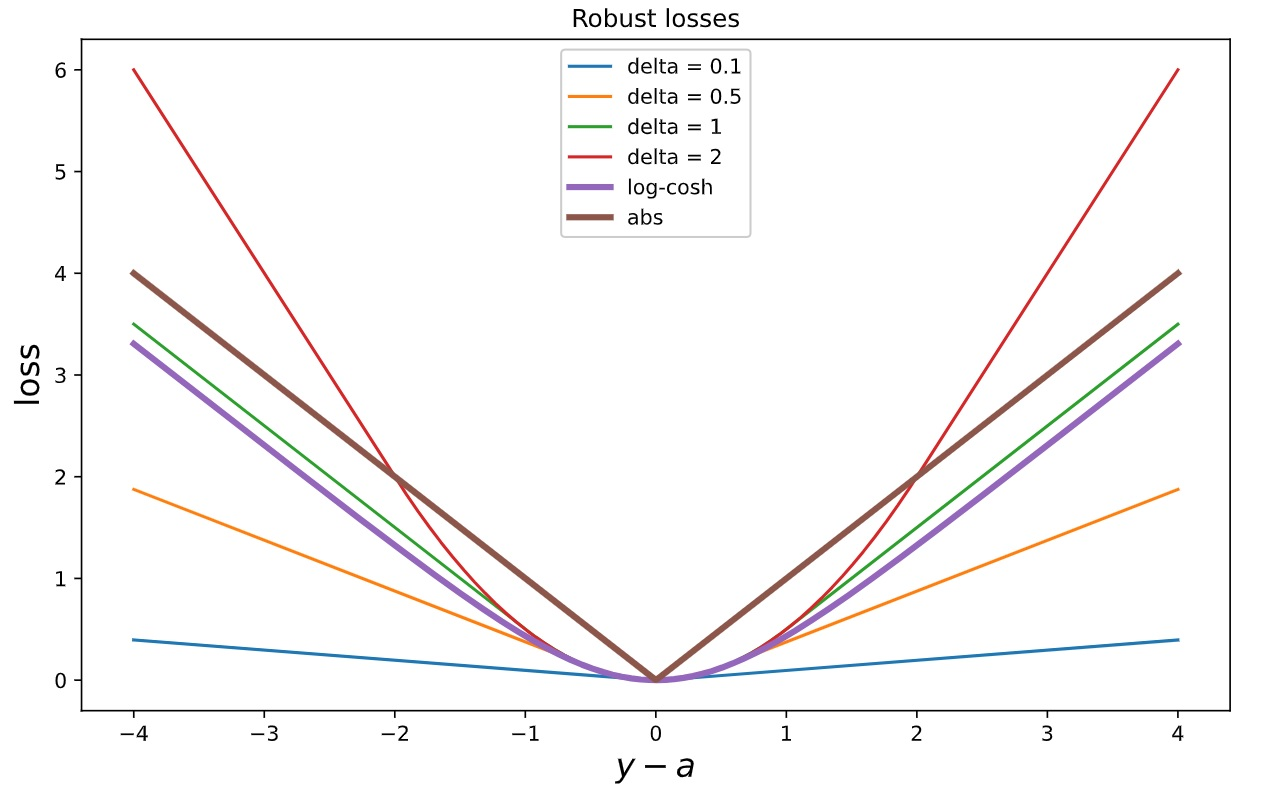
\includegraphics[width=0.7\linewidth]{loss_func.jpg}
	
	\caption{Визуализация функций потерь}
	
	\label{fig:loss_func}
	
\end{figure}

\subsubsection{Оценивание качества модели}

Для оценки качества исследуемой модели размеченные данные разделяются на две части: обучающую и контрольную выборки. На первой будет происходить обучение модели, на второй будем производить тестирование. Так как результат существенно зависит от разбиения данных, размеченные данные разбиваются на $k$ блоков $X_1, \dots, X_k$ примерно одинакового размера. После чего обучается $k$ моделей $a_1(x), \dots, a_k(x)$, причем $i$-я модель обучается на всех объектах кроме блока $i$. После этого качество модели оценивается по тому блоку, который не участвовал в обучении, а результат усредняется:
 \begin{gather}\label{modelquality}
	CV = \frac{1}{k}\sum\limits_{i=1}^{k}Q(a_i(x), X_i).
\end{gather}

Заметим, что в нашей задаче данные имеют структуру временного ряда, поэтому случайно их перемешивать будет некорректно. Решением этой проблемы может быть подход \textbf{time series cross validation}.

Суть метода заключается в том, что мы начинаем обучать модель на небольшом отрезке временного ряда от начала до некоторого $t$, затем делаем прогноз на $t+n$ и считаем ошибку. На следующем шаге расширяем обучающую выборку до $t+n$ и прогнозируем с $t+n$ до $t+2n$. Так мы продолжаем сдвигать тестовый отрезок ряда до тех пор пока не достигнем последнее доступное наблюдение. Схематически логику можно представить так (рис.~\ref{fig:tcross_val}). 

\begin{figure}[h]
	
	\centering
	
	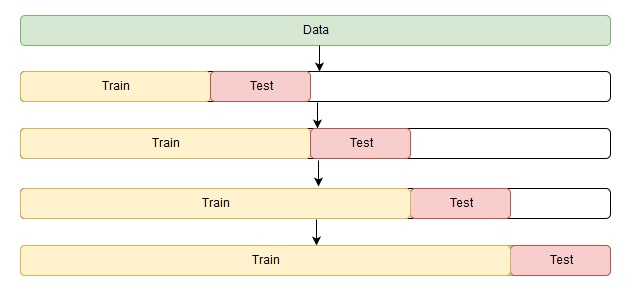
\includegraphics[width=0.7\linewidth]{tcross_val.jpg}
	
	\caption{Кроссвалидация временного ряда}
	
	\label{fig:tcross_val}
	
\end{figure}

\subsubsection{Обучение линейной регрессии}

Довольно распространенный способ обучения линейной регрессии с использованием среднеквадратичной ошибки. В этом случае получаем задачу оптимизации:
 \begin{gather}\label{linreglearn1}
	\frac{1}{l}\sum\limits_{i=1}^{l}(\langle\omega, x_i\rangle - y_i)^2 \rightarrow \min_{\omega}.
\end{gather}
Пусть $X$~--- это матрица "объекты-признаки"\, $y$~--- вектор ответов, $\omega$~--- вектор параметров, тогда задачу можно переписать в матричном виде:
 \begin{gather}\label{linreglearn2}
	\frac{1}{l}\|X\omega - y\|^2 \rightarrow \min_{\omega},
\end{gather}
здесь используется обычная $L_2$-норма. Если найти экстремум данного функционала, получим:
 \begin{gather}\label{linreglearn3}
	\omega = (X^TX)^{-1}X^Ty.
\end{gather}
Безусловно наличие явной формулы для оптимального веса векторов является большим преимуществом линейной регрессии с квадратичным функционалом. Но данная формула не всегда применима. Так обращение матрицы $X$~--- это сложная операция с кубической сложностью от количества признаков, данная проблема решается использованием линейных методов оптимизации. Но также матрица $X^TX$ может быть вырожденной или плохо обусловленной, данную проблему приходится решать регуляризацией.

Вывод аналитических формул в машинном обучении редко выполним, поэтому был разработан подход, в рамках которого модель можно обучать для широкого класса функционалов.

\subsubsection{Градиентный спуск}

Оптимизационные задачи вида \ref{linreglearn2} можно решать итерационно с помощью градиентных методов. Основное свойство антиградиента~--- указывать направление наискорейшего убывания функции в точке. Пусть $\omega^{(0)}$~--- начальный набор параметров, который можно задать нулевым или сгенерировать случайным образом. Градиентный спуск заключается в повторении следующих шагов до сходимости:
 \begin{gather}\label{gradmet1}
	\omega^{(k)} = \omega^{(k-1)} - \eta_k\nabla Q (\omega^{(k-1)}),
\end{gather}
где $Q(\omega)$~--- значение функционала ошибки для набора параметров $\omega$, $\eta_k$~--- длина шага, которая позволяет контролировать скорость движения.

Останавливать схождение итерационного процесса можно, например, при близости градиента к нулю или при слишком малом изменении вектора весов. Для градиентного спуска имеет место следующая оценка сходимости:
 \begin{gather}\label{gradmet2}
	Q(\omega^{(k)})-Q(\omega^*) = O\left(\frac{1}{k}\right).
\end{gather}

\subsubsection{Градиентный бустинг}

В основе этого подхода лежит идея комбинирования нескольких моделей для получения более точного результата. Ансамблем называется набор предсказателей, которые вместе дают результат. Ансамбль, в котором предсказатели выстроены последовательно, называется бустинг. Градиентный бустинг~--- это техника машинного обучения для задач классификации и регрессии, которая строит модель предсказания в форме ансамбля базовых предсказывающих моделей, чаще всего решающих деревьев. 

Для начала рассмотрим \textbf{применение бустинга в задаче регрессии}, а именно обратимся к задаче минимизации квадратичного функционала:

 \begin{gather}\label{bust1}
	\frac{1}{2}\sum\limits_{i=1}^{l}(a(x_i)-y_i)^2 \rightarrow \min_a
\end{gather}

Итоговый алгоритм будем искать в виде суммы базовых моделей $b_n(x)$:
\begin{gather}\label{bust2}
	a_N(x) = \sum\limits_{i=1}^{N}b_n(x),~~b_n\in \mathcal{A}.
\end{gather}

Построим первый базовый алгоритм:
\begin{gather}\label{bust3}
	b_1(x): = \argmin_{b\in\mathcal{A}}\frac{1}{2}\sum\limits_{i=1}^{l}(b(x_i)-y_i)^2.
\end{gather}

Для большинства семейств алгоритмов эта задача решается просто. Далее необходимо рассчитать остатки на каждом объекте~--- расстояния от ответа алгоритма до истинного ответа:
\begin{gather}\label{bust4}
	s_i^{(1)} = y_i - b_1(x_i).
\end{gather}
Если прибавить эти остатки к ответам на обучающей выборке, то алгоритм не будет допускать ошибок на обучающей выборке. Поэтому будет разумно построить второй алгоритм, таким образом, чтобы его ответы были как можно ближе к остаткам:
\begin{gather}\label{bust5}
	b_2(x): = \argmin_{b\in\mathcal{A}}\frac{1}{2}\sum\limits_{i=1}^{l}(b(x_i)-s_i^{(1)})^2.
\end{gather}
И так далее каждый следующий алгоритм будем настраивать на остатки предыдущих:
\begin{gather}\label{bust6}
	s_i^{(N)} = y_i - \sum\limits_{n=1}^{N-1}b_n(x_i) = y_i - a_{N-1}(x_i),~~~~i=1,\dots,l;
	\\
	b_N(x): = \argmin_{b\in\mathcal{A}}\frac{1}{2}\sum\limits_{i=1}^{l}(b(x_i)-s_i^{(N)})^2.
\end{gather}
Стоит отметить и тот факт, что остатки могут быть найдены как антиградиент функции потерь по ответу модели, посчитанный в точке ответа уже построенной композиции:
\begin{gather}\label{bust7}
	s_i^{(N)} = y_i - a_{N-1}(x_i) = - \frac{\partial }{\partial z}\frac{1}{2}(z-y_i)^2\bigg|_{z=a_{N-1}(x_i)}
\end{gather}

Получается, что выбирается такой базовый алгоритм, который как можно сильнее уменьшит ошибку композиции, так как он близок к антиградиенту функционала на обучающей выборке. Рассмотрим это свойство подробнее, а также обобщим его на другие функции потерь.

\textbf{Градиентный бустинг.} Рассмотрим некоторую дифференцируемую функцию потерь $L(y,z)$. Будем строить взвешенную сумму базовых алгоритмов:
\begin{gather}\label{gradbust1}
	a_N(x) = \sum\limits_{n=0}^{N}\gamma_nb_n(x), 
\end{gather}
где $b_0(x)$~--- начальный базовый алгоритм, как правило коэффициент при нем берут равным единице, а сам алгоритм выбирают максимально простым, для задач регрессии это обычно средний ответ:
\begin{gather}\label{gradbust2}
	b_0(x) =  \frac{1}{l}\sum\limits_{i=1}^{l}y_i.
\end{gather}

Применим индукционный подход и предположим, что мы построили композицию $a_{N-1}(x)$ из $N-1$ алгоритма, и хотим теперь выбрать следующий базовый алгоритм $b_N(x)$ таким образом, чтобы как можно сильнее уменьшить ошибку:
\begin{gather}\label{gradbust3}
	\sum\limits_{i=1}^{l}L(y_i, a_{N-1}(x_i)+\gamma_Nb_N(x_i)) \rightarrow \min_{b_N, \gamma_N}.
\end{gather}

Для решения этой задачи предположим, что в качестве алгоритма $b_N(x)$ мы могли бы рассмотреть произвольную функцию, тогда задача сводится к необходимости понять какие значения $s_i$ она должна принимать на  объектах обучающей выборки:
\begin{gather}\label{gradbust4}
	\sum\limits_{i=1}^{l}L(y_i, a_{N-1}(x_i)+s_i) \rightarrow \min_{s_1, \dots, s_l}.
\end{gather}

Конечно, можно потребовать $s_i = y_i-a_{N-1}(x_i)$, но такой подход никак не учитывает особенности функции потерь $L(y,z)$, поэтому правильнее предложить $s_i$ противоположным производной функции потерь в точке $z=a_{N-1}(x_i)$:
\begin{gather}\label{gradbust5}
	s_i = -\frac{\partial L}{\partial z}\bigg|_{z = a_{N-1}(x_i)}.
\end{gather}

При таком подходе мы сдвинемся в сторону скорейшего убывания функции потерь. При этом интересным свойством оказывается совпадение вектора сдвигов $s = (s_1,\dots, s_l)$ с антиградиентом:
\begin{gather}\label{gradbust6}
	\left(-\frac{\partial L}{\partial z}\bigg|_{z = a_{N-1}(x_i)}\right)_{i=1}^{l} = -\nabla_z\sum\limits_{i=1}^{l}L(y_i, z_i)|_{z_i = a_{N-1}(x_i)}.
\end{gather}
При таком выборе сдвигов по сути происходит один шаг градиентного спуска, при движении в сторону наискорейшего убывания ошибки на обучающей выборке. Речь идет о градиентном спуске в $l$-мерном пространстве предсказаний алгоритма на объектах обучающей выборки. 

Теперь, когда есть понимание, какие значения должен принимать новый алгоритм на обучающей выборке необходимо по данным значениям, заданным в конечном числе точек построить функцию определенную на всем пространстве объектов. По сути это решение классической задачи обучения с учителем, воспользуемся простым функционалом, а именно среднеквадратичной ошибкой, для построения базового алгоритма, приближающего градиент функции потерь на обучающей выборке:
\begin{gather}\label{gradbust7}
	b_N(x) = \argmin_{b\in\mathcal{A}} \sum\limits_{i=1}^{l}(b(x_i)-s_i)^2.
\end{gather}
Важно, что на этом шаге мы оптимизируем функцию потерь независимо от функционала исходной задачи, так как вся информация о функции потерь $L$ находится в антиградиенте 
$s_i$ и на данном шаге решается лишь задача аппроксимации функции по $l$ точкам. Естественно можно использовать и другие функционалы, но среднеквадратичной ошибки обычно оказывается достаточно. 

После того, как новый базовый алгоритм найден, можно подобрать коэффициент при нем по аналогии с наискорейшим градиентным спуском:
\begin{gather}\label{gradbust8}
\gamma_N = \argmin_{\gamma\in\mathbb{R}}\sum\limits_{i=1}^{l}L(y_i, a_{N-1}(x_i) + \gamma b_N(x_i)).
\end{gather}

Подход с аппроксимацией антиградиента базовыми алгоритмами, описанный выше, и называется градиентным бустингом. Данный метод представляет собой поиск лучшей функции, восстанавливающей зависимость ответов от объектов, в пространстве всех возможных функций. Поиск этой функции происходит с помощью псевдоградиентного спуска, каждый шаг делается вдоль направления, задаваемого некоторым базовым алгоритмом. При этом сам базовый алгоритм выбирается так, чтобы как можно лучше приближать антиградиент ошибки на обучающей выборке.  

\subsubsection{Нейронные сети}
Для начала необходимо определить понятие нейрона в машинном обучении. Пусть на вход подается $n$ величин $x_1,\dots, x_n$ бинарных признаков, описывающих объект $x$. Эти признаки будем трактовать как импульсы, поступающие на вход нейрона через $n$ входных каналов. Будем считать, что импульсы попадая в нейрон складываются с весами $\omega_1,\dots,\omega_n$. Если суммарный импульс превышает заданный порог активации $\omega_0$, то нейрон возбуждается и выдает на выходе один результат, иначе другой, в основе выбора лежит функция активации. Таким образом работу нейрона можно представить как вычисление функции:
\begin{gather}\label{ney1}
	a(x,\omega) = \sigma(\langle \omega, x \rangle) = \sigma\left(\sum\limits_{i=1}^{n} \omega_if_i(x)-\omega_0, \right)
\end{gather}
где $\sigma(z)$~--- функция активации, схематично принцип работы нейрона изображен на (рис.~\ref{fig:neyron}).

\begin{figure}[h]
	
	\centering
	
	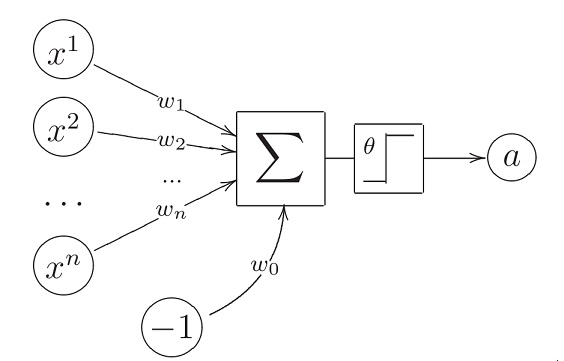
\includegraphics[width=0.5\linewidth]{neyron.jpg}
	
	\caption{Нейрон}
	
	\label{fig:neyron}
	
\end{figure}

Нейронной сетью называется композиция таких нейронов и визуально может быть представлена следующим образом (рис.~\ref{fig:neyron_net}).
\begin{figure}[h]
	
	\centering
	
	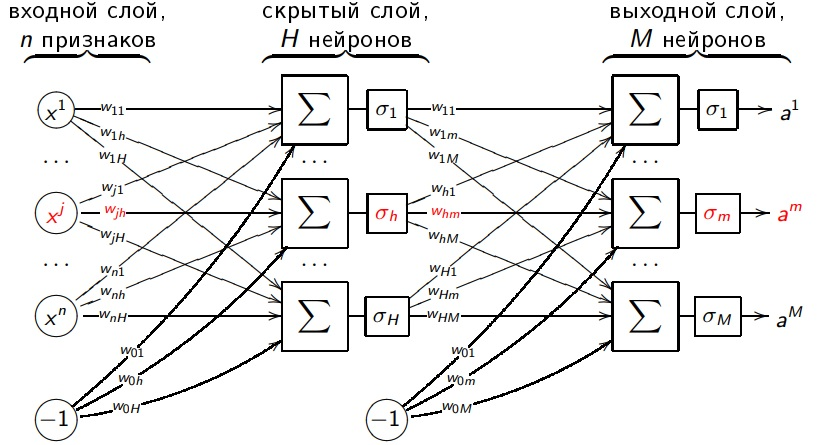
\includegraphics[width=0.8\linewidth]{neyron_net.jpg}
	
	\caption{Нейронная сеть}
	
	\label{fig:neyron_net}
	
\end{figure}

Обучение нейронной сети в задачах регрессии схоже с градиентным спуском. Пусть $\{x_i, y_i\}_{i=1}^{N}$~--- обучающая выборка, $a(x,\omega)$~--- исследуемая нейросетевая модель, $L(y,z)$~--- функция потерь, тогда задача обучения может быть представлена, как:
\begin{gather}\label{ney2}
	Q(\omega) = \sum\limits_{i=1}^{N}L(y_i, a(x_i, \omega)) \rightarrow \min_{\omega}.
\end{gather}

Важным преимуществами нейросетевых алгоритмов является возможно наделять архитектуру сети нужными свойствами, принимать на входе и генерировать на выходе сложно структурированные данные. Однако, архитектуру необходимо подбирать вручную и моделям свойственно сильное переобучение. Нейронные сети хорошо подходят для решения задач на однородных входных данных, например изображениях. При регрессии на неоднородных табличных данных при применении классических моделей показывают не лучший результат согласно исследованиям \ref{}, исследование работы нейросетевых моделей в рамках данной работы не проводилось.

\subsection{Обзор алгоритмов  кластеризации в машинном обучении}

Пусть дана выборка объектов $X = (x_i)_{i-1}^{l},~x_i\in\mathbb{X}$. Задача кластеризации заключается в том, чтобы необходимо выявить в данных $K$ кластеров~--- таких областей, что объекты внутри одного кластера похожи друг на друга, а из разных кластеров нет. Если определять задачу формально, то требуется построить алгоритм $a: \mathbb{X}\rightarrow{1,\dots,K}$ , определяющий для каждого объекта номер его кластера.

\subsubsection{Метрики качества кластеризации}
Подходы к оценке качества кластеризации можно разделить на два ключевых: внутренний и внешний. В основе внутреннего лежат некоторые свойства выборки и кластеров, а внешнего на некоторых дополнительных данных, например информации об истинных кластерах.

Если известно истинное распределение объектов по кластерам, то задачу можно рассматривать как многоклассовую классификацию. Так как в текущем исследовании эталонных данных о распределении нет, то этот подход далее рассмотрен не будет.

Далее будут рассмотрены внутренние метрики качества. 

\textbf{Внутриклассовое расстояние}:
\begin{gather}\label{klastdist1}
	\sum\limits_{k=1}^{K}\sum\limits_{i=1}^{l}[a(x_i)=k]\rho(x_i, c_k),
\end{gather}
где $c_k$~--- центр кластера, $\rho(x,z)$~--- некоторая функция расстояния. Этот функционал требуется минимизировать.

\textbf{Межклассовое расстояние}:
\begin{gather}\label{klastdist2}
\sum\limits_{i,j = 1}^{l}[a(x_i)\not=a(x_j)]\rho(x_i, x_j).
\end{gather}
Этот функционал необходимо максимизировать.

\textbf{Индекс Данна}:
\begin{gather}\label{klastdist3}
	\frac{min_{1\leq k\leq k'\leq K}d(k,k')}{max_{1\leq k\leq K}d(k)}, 
\end{gather}
где $d(k,k')$~--- расстояние между кластерами $k$ и $k'$, например можно взять евклидово расстояние между центрами, а $d(k)$~--- внутрикластерное расстояние для $k$-го кластера. Данный индекс необходимо максимизировать.

\subsubsection{Метод $k$-средних}

Одним из наиболее популярных методов кластеризации является $K-Means$, который оптимизирует внутрикластерное расстояние \ref{klastdist1}, используя квадрат евклидовой метрики. В данном функционале две степени свободы: центры кластеров $c_k$ и распределение объектов по кластерам $a(x_i)$. Выберем для этих величин произвольные начальные приближения, а затем пошагово будем их оптимизировать.

Фиксируем центры кластеров, внутрикластерное расстояние будет минимальным при условии, что каждый объект будет будет относится к тому кластеру, чей центр является ближайшим:
\begin{gather}\label{klastdist4}
	a(x_i) = \argmin_{1\leq k\leq K} \rho(x_i, c_k).
\end{gather}

Фиксируем распределение объектов по кластерам. После чего внутрикластерное расстояние с квадратом евклидовой можно продифференцировать по центрам кластеров и вывести аналогичные формулы для них:
\begin{gather}\label{klastdist5}
c_k = \frac{1}{\sum\limits_{i=1}^{l}[a(x_i)= k]} \sum\limits_{i=1}^{l}[a(x_i)= k]x_i.
\end{gather}
Повторяя эти шаги до сходимости, алгоритм выдает распределение объектов по кластерам. Стоит отметить, что результат работы $k-means$ существенно зависит от начального приближения

\subsubsection{Иерархическая кластеризация}
Описанный выше метод кластеризации имеет плоскую структуру кластеров. Для части задач бывает необходимо построить иерархию вложенных кластеров,в которой верхним уровнем является один большой кластер, а на нижнем уровне $l$ кластеров, состоящих из 1 объекта каждый. Одним из таких подходов является восходящая кластеризация, на нижнем уровне все объекты принадлежат к отдельным кластерам:$C^l = \{\{x_1\},\dots,\{x_l\}\}$. Каждый следующий уровень $C^j$ получается путем объединения двух наиболее похожих кластеров с предыдущего уровня $C^{j+1}= \{X_1, \dots,X_{j+1}\}$. При этом схожесть кластеров можно определять с помощью некоторой функции $d(X_m, X_n)$, например это может быть расстояние между центрами кластеров.

%%%%%%%%%%%%%%%%%%%%%%%%%%%%%%%%%%%%%%%%%%%%%%%%%%%%%%

\newpage
\section{Предлагаемые изменения}
На фоне обостренной быстро меняющейся экономической ситуации в стране, а также крупных логистических проблем в строительной отрасли, мониторинг финансируемых объектов стройки, по которым банк является гарантом, важен как никогда.
Поэтому для понимания необходимости заложения резервов по строительным объектам и прогноза соответствия фактических работ по строительному объекту и план-графиков, необходимо оценивать фактическую степень готовности объекта. Как унифицированный параметр-индикатор в данном исследовании предлагается дата полной готовности объекта.   

\subsection{Формальная постановка задачи}

Необходимо спрогнозировать фактическую дату готовности строительного объекта на отчетную дату на основании актуальных данных об объекте строительства и девелопере. Так как прогноз значения с календарным типом данных является затруднительным, будем прогнозировать число дней, которое пройдет с отчетной даты до даты готовности. Прогноз будет реализован с применением алгоритмов машинного обучения.

В качестве критериев оценки качества работы алгоритмов предлагается сравнение ошибок: MSE, $R^2$, MAE и MAPE.

\subsection{Входные данные}

В роли основного источника данных выступает закрытое внутреннее корпоративное хранилище данных "ПАО Сбербанк" (рис.~\ref{fig:data_source}) Sber Data Factory или Фабрика данных. Данные, интересующие нас в рамках решаемой задачи,  реплицируются из трех основных источников: Единой информационной системы жилищного строительства (ЕИСЖС), Единого ресурса застройщиков (ЕРЗ) и внутрибанковских сервисов. Из последних тянется количественная аналитика по объектам ипотеки, эскроу счетов и проектному финансированию. Единый ресурс застройщиков предлагает агрегированные данные продаж, собраные на базе статистики агенств и самих девелоперов. ДОМ.РФ же при подключении к Api ЕИСЖС  предлагает некоторые аналитические данные собраные на базе собственных моделей и статистики дочернего банка Банк ДОМ.РФ, а также набор данных, представленных на открытом портале наш.дом.рф. Последние в обязательном порядке поставляются застройщиками в виде соответствующих документов: проектных деклараций, разрешительной документации, проектной документации и отчетности застройщика. 
Здесь важно заметить, что в проектной декларации, публикуемой ежемесячно, фигурирует дата планового окончания строительства, прогнозируемая застройщиком. Эта дата будет выбрана в качестве значений для обучающей выборки.  

Обработка данных выполнена при помощи Jupyter Notebook на языке программирования python.

\begin{figure}[h]
	
	\centering
	
	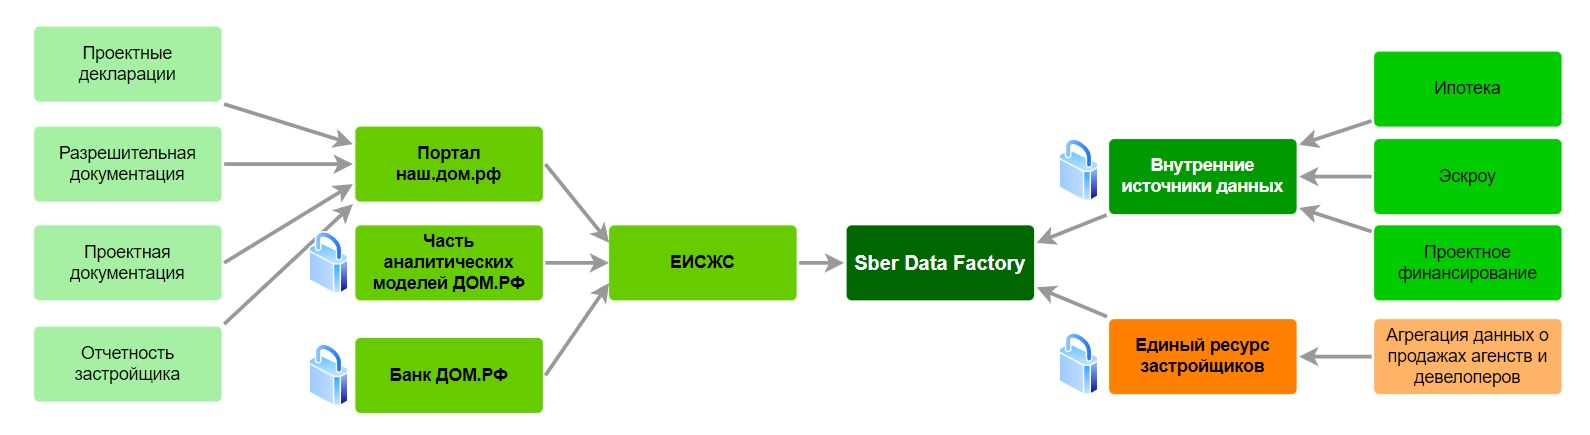
\includegraphics[width=\linewidth]{data_source.jpg}
	
	\caption{Схема источников данных}
	
	\label{fig:data_source}
	
\end{figure}

Данные из всех систем связываются по ключевым идентификаторам и сджойниваются в одну матрицу признаков посредством системы работы с данным Hadoop.

\subsection{Описание моделей}

В данном исследовании сравнивается результат работы двух аналитических прогнозных модели машинного обучения: линейной регрессии и градиентного бустинга.
Также для каждой из моделей проверяется гипотеза эффективности применения предварительной кластеризации объектов строительства. Схематичное изображение дата-тракта исследованных моделей представлено на (рис.~\ref{fig:data_tract}).

 
\begin{figure}[h]
	
	\centering
	
	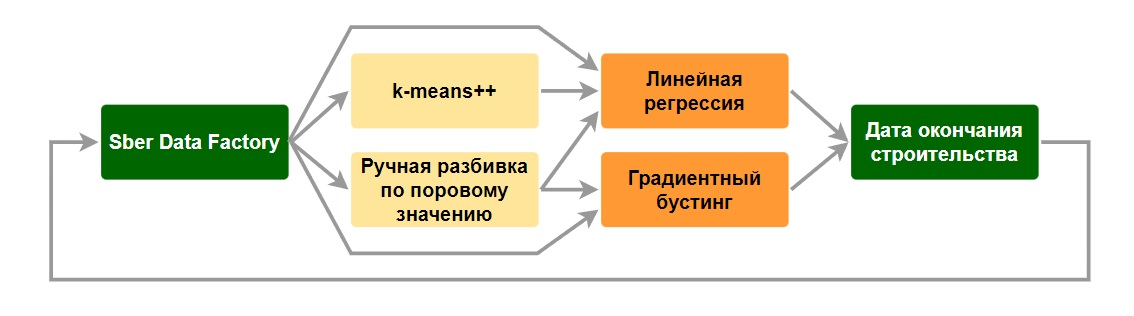
\includegraphics[width=\linewidth]{data_tract.jpg}
	
	\caption{Схематичное изображение исследованных моделей}
	
	\label{fig:data_tract}
	
\end{figure} 
 
 
 
\subsubsection{Этап предобработки данных}
 
На этапе предобработки данных исследовалась гипотеза, о возможности сгруппировать каким-либо образом объекты строительства для коллективного анализа и применения корректирующих мер на схожие объекты. 

В качестве группирующих алгоритмов использовались алгоритм кластеризации $k-means^{++}$ и классификация по порогу фильтрующего значения.

\textbf{$\mathbf{k-means^{++}}$.} Реализация алгоритма взята из библиотеки sklearn с модификацией выбора первого приближения. Алгоритм кластеризации неплохо себя показал, однако потребовал дополнительного времени для обучения. Кластеризация производилась с входным параметром 3, 4, и 5, задающим предполагаемое количество кластеров. Такие значения подобраны из соображений дальнейшей работы с моделями. Обслуживать более 5 регрессионных моделей сложно, а при количестве меньшем 3 кластеризация теряет смысл исходя из природы данных.
Результат работы алгоритма представлен на (рис.~\ref{fig:k-means}), взята наиболее репрезентативная проекция, координаты не интерпретируемы. Однако видна тенденция к удачному разделению множества объектов на 4 группы это подтверждают и количественные метрики оценки ошибки в Таблице~\ref{Tab:2}. Ввиду большого набора признаков в исходном датасете и небольшого количества объектов определить степень влияния конкретного признака на попадание объекта в тот или иной кластер становится проблематично, что снижает общую интерпретируемость модели. 

\begin{figure}[h]
	
	\centering
	
	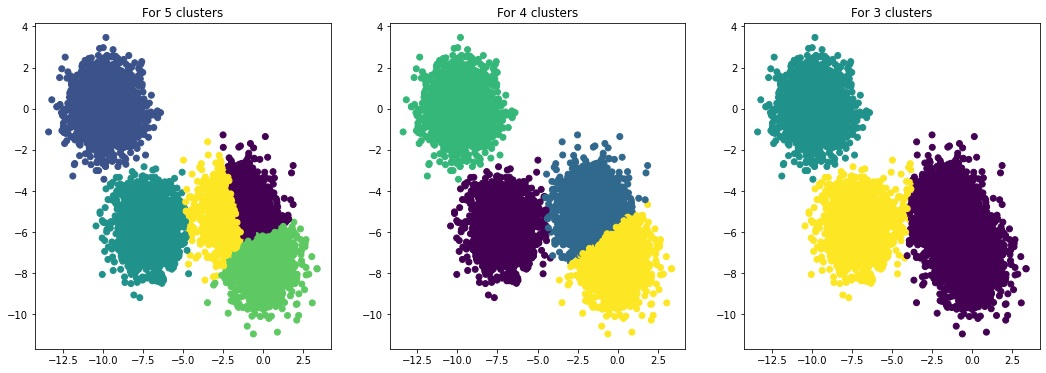
\includegraphics[width=0.8\linewidth]{k-means.jpg}
	
	\caption{Результат работы k-means для разного количества кластеров}
	
	\label{fig:k-means}
	
\end{figure} 

\begin{table}[h]
	\centering
	%\begin{tabular}{l|l|l|l}
	\begin{tabular}{cccc}
		
		\hline  Модель& \specialcell{Внутреннее\\расстояние} &  \specialcell{Внешнее\\расстояние} & \specialcell{Индекс\\Данна} \\
		\hline $k-means^{++}$ 5  & 18,7 & 28,9 & 1,15\\
		$k-means^{++}$ 4 & 15,9 & 28,1 & 1,31\\
		$k-means^{++}$ 3 & 19,4 &  23,9 & 1,05\\
		\hline
		\textbf{Пороговая классификация}&  \textbf{20,2}& \textbf{27,4}& \textbf{1,23}   \\
		\hline 
	\end{tabular}
	
	\caption{Сравнение метрик качества $k-means^{++}$ для разного количества кластеров}
	\label{Tab:2}
\end{table}


\textbf{Пороговая классификация.} Здесь, проверялась гипотеза о возможности разделить объекты недвижимости по уровню, а именно, за основу был взят признак $f$:
\begin{gather}\label{pklas1}
	a_i\leq \frac{p_j\cdot|R|}{\sum\limits_{k\in R} p_k}\leq a_{i+1},
\end{gather}
где $p_j$~--- актуальная стоимость строительства исследуемого объекта, $R$~--- все объекты жилищного строительства в регионе, $|R|$~--- количество этих объектов, а $a_i$~--- выведенные эмпирически пороговые значения. Таким образом, по сути объект строительства оценивается по отношению стоимости его строительства к стоимости среднего объекта стройки в регионе, и на основе пороговых значений этого признака происходит классификация. На (рис.~\ref{fig:porclas}) представлена визуализация значения признака оценки. Не трудно заметить, что точки можно удачно разделить на 4 группы. На основе данных были выбраны 3 пороговых значения по центрам отрезков крайних точек групп: $a_1 \approx 0,8; a_2 \approx 1,2; a_3 \approx 1,5$.

Заметим, что величины ошибок для этого подхода не сильно хуже результатов работы алгоритмов кластеризации (Таблица~\ref{Tab:2}). Однако, интерпретируемость пороговой классификации значительно выше, так выделяются 4 слоя объектов строительства, условно их можно назвать: "эконом", "средний класс", "бизнес" и "элитное" жилье. Интерпретируемость высока еще и потому, что такой терминологии придерживаются маркетологи крупных девелоперских компаний. 

Резюмируя, разница в величине ошибки $\approx10\%$ на данном этапе не является критической, так как напрямую не влияет на точность модели, а только на то, в какую регрессионную группу попадет объект. Поэтому на данном этапе в силу лучшей интерпретируемости предполагаем использование модели классификации с большим приоритетом.  

\begin{figure}[h]
	
	\centering
	
	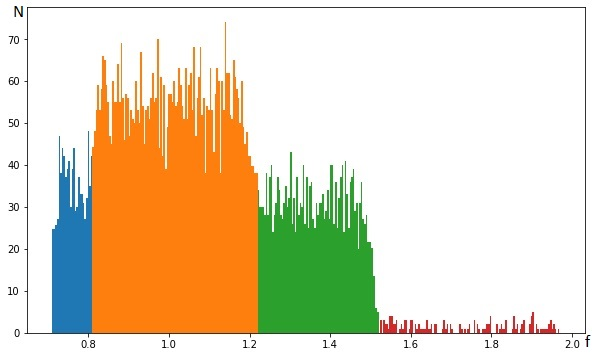
\includegraphics[width=0.8\linewidth]{porclas.jpg}
	
	\caption{Распределение значений признака $f$ }
	
	\label{fig:porclas}
	
\end{figure} 


\subsubsection{Ядро модели}

%%%%%%%%%%%%%%%%%%%%%%%%%%%%%%%%%%%%%%%%%%%%%%%%%%%%%

\newpage
\section{Результаты работы алгоритма}
\subsection{Пример полученных результатов - ключевые атрибуты}

\subsection{Сравнение результатов с другими методами}

\subsection{Сравнение результатов с оценкой предложенной метрики качества}


%%%%%%%%%%%%%%%%%%%%%%%%%%%%%%%%%%%%%%%%%%%%%%%%%%%%%

\newpage
\section{Экономический эффект от внедрения модели}

%%%%%%%%%%%%%%%%%%%%%%%%%%%%%%%%%%%%%%%%%%%%%%%%%%%%%


\newpage
\section{Заключение}



%%%%%%%%%%%%%%%%%%%%%%%%%%%%%%%%%%%%%%%%%%%%%%%%%%%%%


\newpage

\bibliographystyle{gost71s}
\bibliography{mylib}
\nocite{GV}

\end{document}